\documentclass[10pt,a4paper]{report}
\usepackage[utf8]{inputenc}
\usepackage[spanish]{babel}
\usepackage{amsmath}
\usepackage{amsfonts}
\usepackage{amssymb}
\usepackage{graphicx}
\usepackage[document]{ragged2e}
\author{Jose Antonio Garcia Araiza}
\begin{document}
\begin{titlepage}
   \centering
      
\includegraphics[scale=0.25]{11.jpg} \par\vspace{1cm}
      %otra imagen 
      
\includegraphics[scale=0.75]{logos.jpg} \par\vspace{1cm}
   
  	  {\scshape\LARGE Universidad Politécnica de Amozoc\\ \par}
      \vspace{1cm}
 
      {\scshape\large Ingenieria en Software\\ \par}
      \vspace{1cm}
    

   
  		 {\huge\bfseries Analisis de Sistemas\par}
   		 \vspace{2cm}
   		 {\Large\itshape Integrantes: Galileo Ramírez Hernández, José Rene de Lima Camacho, José Antonio Garcia Araiza\par}
         \vspace{1cm}
   		 {\Large\itshape Paulina Centeno Becerra}
         \vfill
         {\Large\bfseries SAPeR\par}
         \vfill
 
\end{titlepage}

%%%%%%%%%%%%%%%%%%%%%%%%%%%%%%%%%%%%%%%%%%%%%%%%%%%%%%%%%%%%%%%%%%%%%%%%%%%%%%%%%%%%%%%%%%%%%%%%%%%%%%%%%
\begin{titlepage}
\begin{flushleft}
{\Large\bfseries \center Indice\par}
\vspace{.5cm}
Introduccion...............................................................
................1\par
 \vspace{1cm}
Resumen...............................................................
......................2\par
 \vspace{1cm}
Objetivo general...............................................................
..........3\par \vspace{1cm}
Objetivos específicos...................................................................
3\par \vspace{1cm}
Desarrollo...................................................................................
8\par \vspace{1cm}
Pruebas......................................................................................
10\par \vspace{1cm}
Anexoss......................................................................................
13\par \vspace{1cm}
Bibliografia.................................................................................
13\par \vspace{1cm}
\end{flushleft}
\end{titlepage}

%%%%%%%%%%%%%%%%%%%%%%%%%%%%%%%%%%%%%%%%%%%%%%%%%%%%%%%%%%%%%%%%%%%%%%%%%%%%%%%%%%%%%%%%%%%%%%%%%%%%%%%%

\begin{titlepage}
{\Large\bfseries Introducción\par}
 \vspace{.5cm}
 \justify
	El sistema que se esta desarrollando esta enfocado a una cadena de restaurantes grande, por lo cual cabe destacar que las ventanas con las que contara son muchas y el tiempo de entrega se estima alrededor de 1 año sin tomar en cuenta posibles cambios.\par 
	\justify
	Lo que se ha trabajado es el modulo del administrador que es uno de los mas importantes ya que sus funciones son muchas, una vez qe se contruyo la base de datos y se preparo lo necesario para trabajar se contruyeron las primeras ventanas y de esta manera una pequeña vista de el comportamiento y funcion del sistema.\par 
	\justify
	Las funciones que podra hacer el administrador seran las siguientes:\par 
	\vspace{.5cm}
	\begin{itemize}
\item{\textbf{Registarse:}\par Es una ventana que permite verificar su acceso por medio de un login.}
\item{\textbf{Dar de Alta:}\par Puede agregar nuevas recetas al menú, un nuevo restaurante y agregar comandas.}
\item{\textbf{Tendra el acceso a la lista de todo lo que maneja su restaurante(aun en desarrollo).}\par}
\end{itemize}
 \vspace{1cm}
\end{titlepage}

%%%%%%%%%%%%%%%%%%%%%%%%%%%%%%%%%%%%%%%%%%%%%%%%%%%%%%%%%%%%%%%%%%%%%%%%%%%%%%%%%%%%%%%%%%%%%%%%%%%%%%%%%

\begin{titlepage}
\begin{flushleft}
{\Large\bfseries Resumen\par}
 \vspace{.5cm}
 \justify
 	El presente documento informa y detalla el comportamiento del modulo de trabajo de el administrador de la cadena del restaurante, es importante destacar que muestra las interfacez en modo beta y no es la vista final que tendra el sistema la idea de las pantallas ya diseñadas es darle una idea al usuario de como se vera el sistema que ha solicitado.\par
 	\justify
 	Los avances que se muetran son los primeros diseños de las ventanas del sistema, una vez analizada la información que proporcione el cliente de cambios y/o modificaciones, se implementaran de manera inmediata en los diseños.
\vspace{1cm}
\end{flushleft}
\end{titlepage}

%%%%%%%%%%%%%%%%%%%%%%%%%%%%%%%%%%%%%%%%%%%%%%%%%%%%%%%%%%%%%%%%%%%%%%%%%%%%%%%%%%%%%%%%%%%%%%%%%%%%%%%%%

\begin{titlepage}
\begin{flushleft}

{\Large\bfseries \center  Objetivo general \par}
 \vspace{2.5cm}
 \justify
\par Implementar un sistema para una cadena de restaurantes que les permita llevar un control sobre los recursos , que los camareros tengan una mayor facilidad al trabajar y puedan brindar un buen servicio para los comensales.\par 
\vspace{3cm}
 \justify
 
 {\Large\bfseries \center Objetivos específicos \par}
 \vspace{2.5cm}
1. Llevar un control y/o sobre los recursos en el almacén.\par 
2. Fácil acceso de reservas para los comensales. \par
3. Facilidad para los camareros a la hora de levantar comanda.\par 
4. Fácil revisión sobre las reservas para el camarero.\par 
\end{flushleft}
\end{titlepage}

%%%%%%%%%%%%%%%%%%%%%%%%%%%%%%%%%%%%%%%%%%%%%%%%%%%%%%%%%%%%%%%%%%%%%%%%%%%%%%%%%%%%%%%%%%%%%%%%%%%%%%%%%%%%%%%%%%%%%%%%%%%%%%%%

\begin{titlepage}
\begin{flushleft}

 \vspace{.5cm}
\section{Ventana de Login}
Su funcion es la de verificar que sea el administrador por medio de su contraseña y su nombre.
\begin{figure}[ht]
\centering
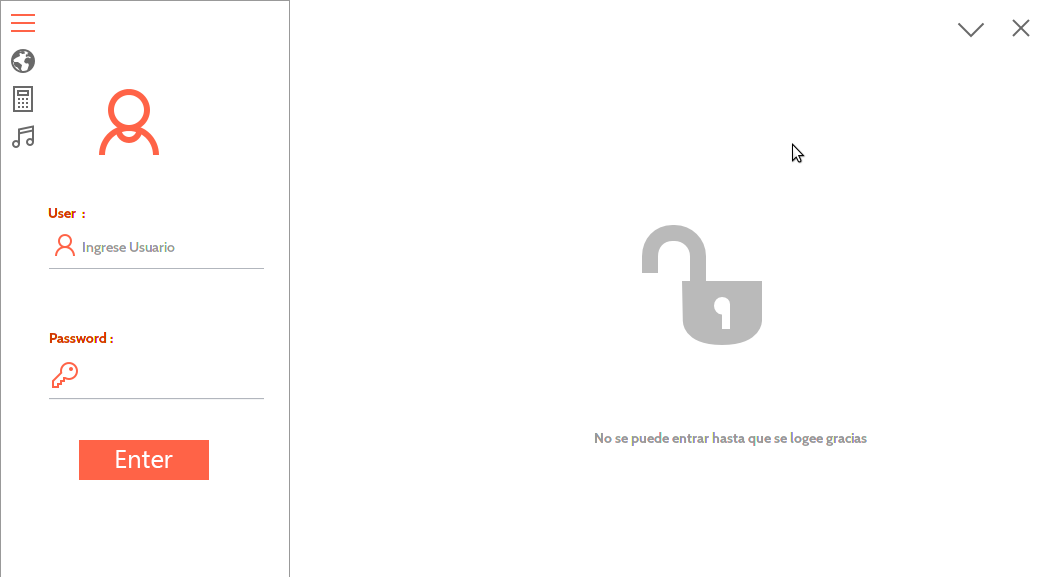
\includegraphics[width=1\textwidth]{loginRestaurante1.png} 
\caption{Exemplo de figura}
\label{fig:figura1}
\end{figure}

\section{Pagina Principal}
Dentro de esta estan dentro todas las opciones que el administrador puede hacer 
\begin{figure}[ht]
\centering
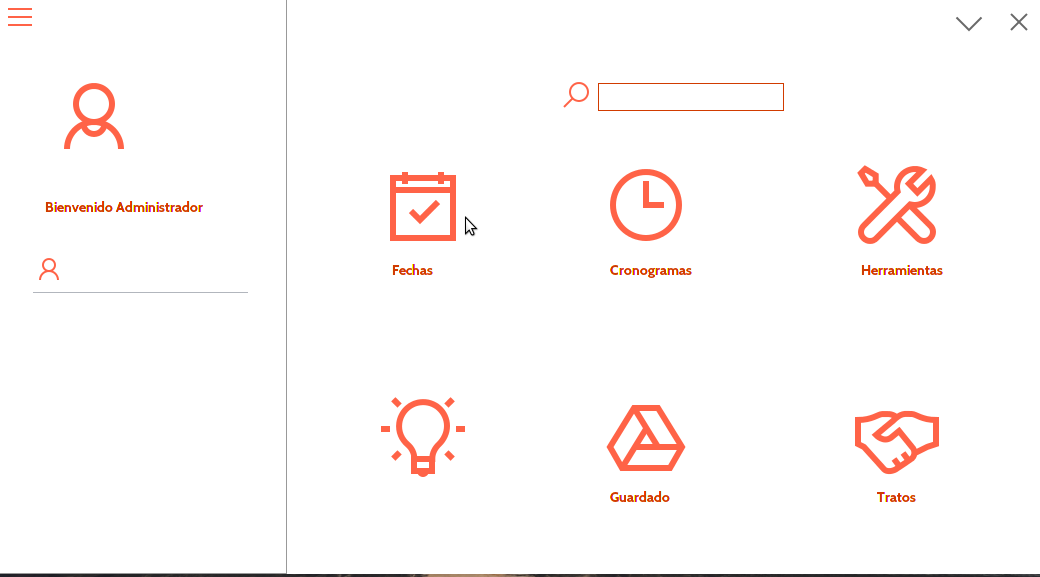
\includegraphics[width=1\textwidth]{indexrestaunrante1.png}

\caption{Exemplo de figura}
\label{fig:figura1}
\end{figure}
	
\vspace{1cm}

\end{flushleft} 
\end{titlepage}

%%%%%%%%%%%%%%%%%%%%%%%%%%%%%%%%%%%%%%%%%%%%%%%%%%%%%%%%%%%%%%%%%%%%%%%%%%%%%%%%%%%%%%%%%%%%%%%%%%%%%%%%%%%%%%%%%%%%%%%%%%%%%%%%

\begin{titlepage}
\begin{flushleft}

\section{Ventana de Alta}
Es un formulario de captura de información(Por el momento aun no esta implementada la nueva Interfas grafica )
\begin{figure}[ht]
\centering
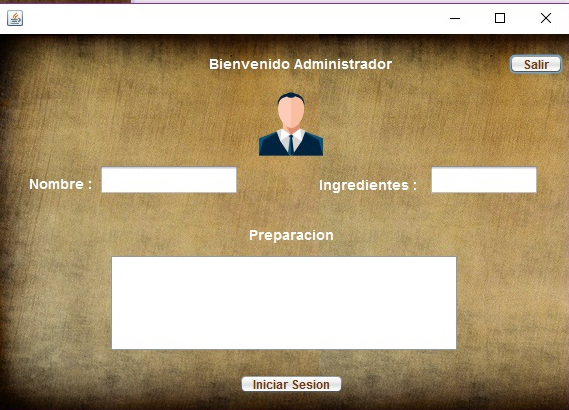
\includegraphics[width=1\textwidth]{41.jpg}
\caption{Exemplo de figura}
\label{fig:figura1}
\end{figure}
	
\vspace{1cm}

\end{flushleft} 
\end{titlepage}

%%%%%%%%%%%%%%%%%%%%%%%%%%%%%%%%%%%%%%%%%%%%%%%%%%%%%%%%%%%%%%%%%%%%%%%%%%%%%%%%%%%%%%%%%%%%%%%%%%%%%%%%%%%%%%%%%%%%%%%%%%%%%%%%

\begin{titlepage}
\begin{flushleft}
 {\Large\bfseries \center  Pruebas  \par}
\section{Ventana de Ingresar Contraseña y Usuario}
Para las pruebas registramos un usuario en la base de datos y despues colocamos la contraseña
\begin{figure}[ht]
\centering
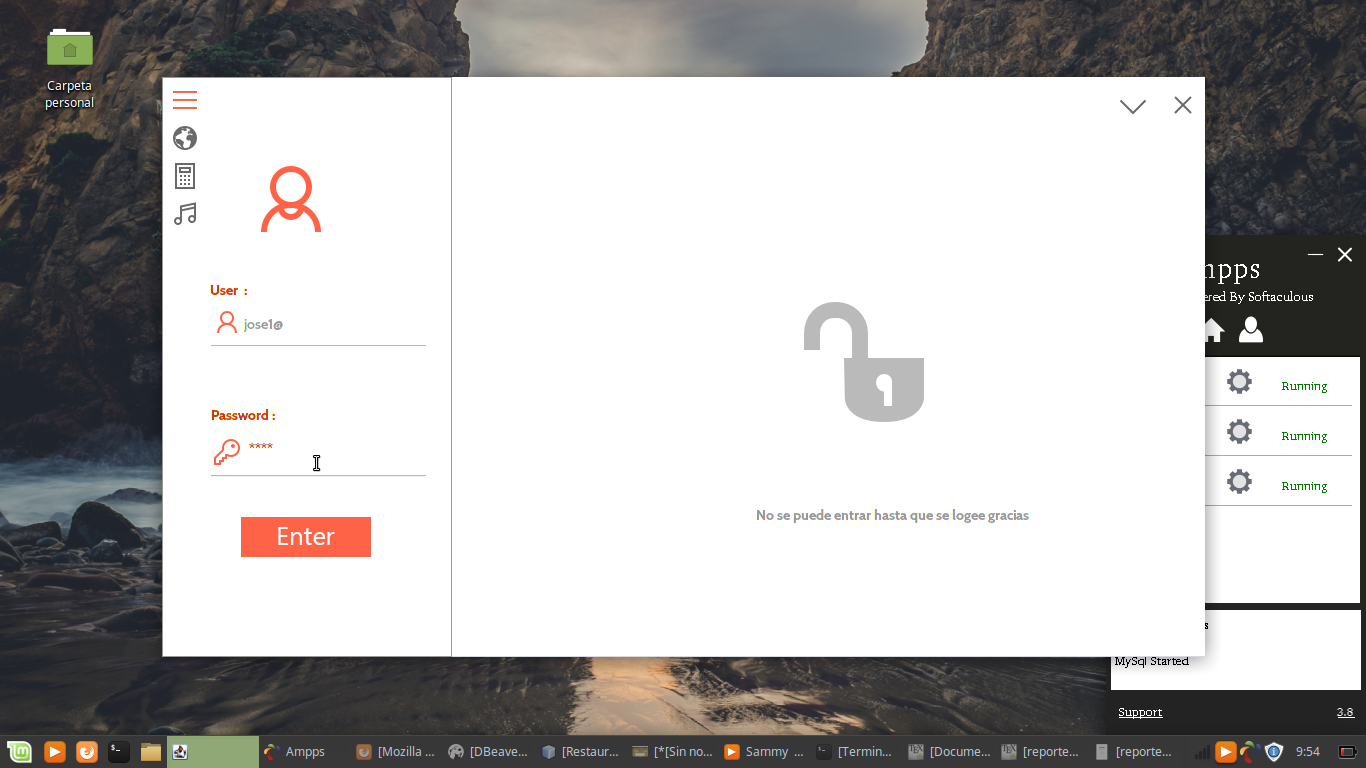
\includegraphics[width=1\textwidth]{17.png}
\caption{Exemplo de figura}
\label{fig:figura1}
\end{figure}
\section{Ventana de Conexion exitosa}
Al Ingresar correctamente el usuario nos mandara un mensaje de conexion exitosa \par
\begin{figure}[ht]
\centering
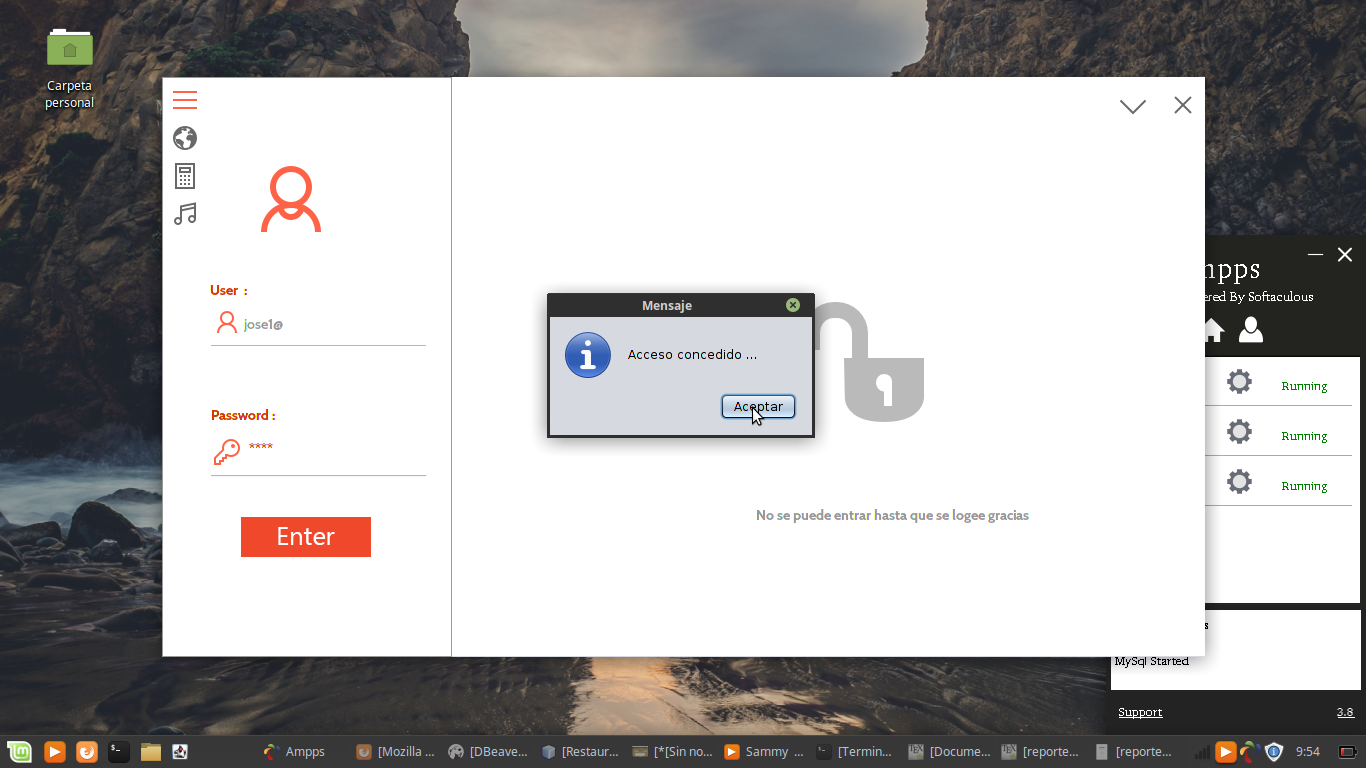
\includegraphics[width=1\textwidth]{18.png}
\caption{Exemplo de figura}
\label{fig:figura1}
\end{figure}
	
\end{flushleft} 
\end{titlepage}

%%%%%%%%%%%%%%%%%%%%%%%%%%%%%%%%%%%%%%%%%%%%%%%%%%%%%%%%%%%%%%%%%%%%%%%%%%%%%%%%%%%%%%%%%%%%%%%%%%%%%%%%%

\begin{titlepage}
\begin{flushleft}
\section{Ventana Inicial}
Al finalizar la conexion exitosa mandara a la pagina principal donde se ingresa el nombre de usario de la base de datos que tengamos \par 
 \vspace{.5cm} 
\begin{figure}[ht]
\centering
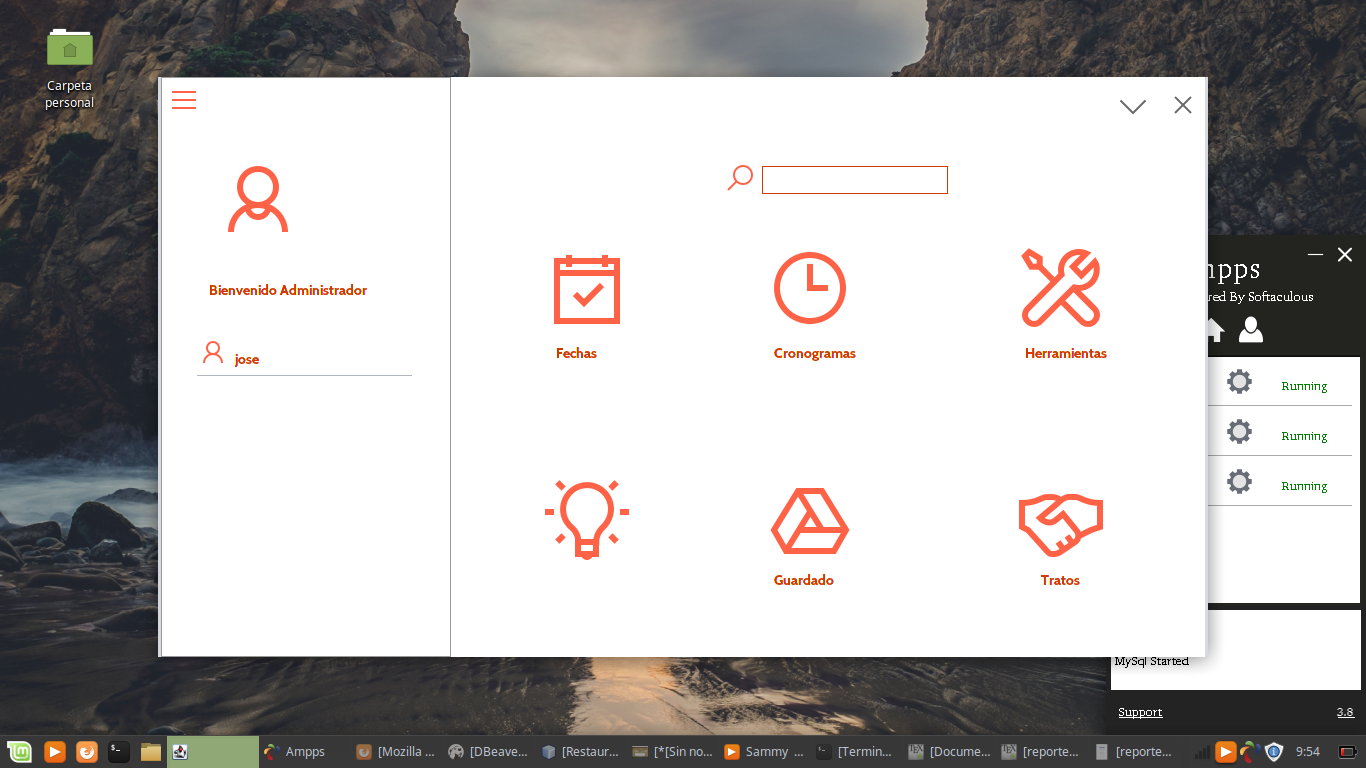
\includegraphics[width=1\textwidth]{19.png}
\caption{Exemplo de figura}
\label{fig:figura1}
\end{figure}

\end{flushleft}
\end{titlepage}

\begin{titlepage}
\begin{titlepage}
{\Large\bfseries \center  Anexos \par}
{\Large\bfseries \center  Vialidades \par}
 \vspace{.5cm}
 \justify
 Existen diferentes tipos de vialidades para analizar antes de empezar a realizar el proyecto, pero ay 3 en partículas que son las fundamentales para que el proyecto pueda ser viable y tenga una buena organización.\\\\
 \vspace{.5cm}
 \justify
--- Vialidad Técnica: Es de mucha ayuda ya que antes de poder implementar el proyecto podemos saber los recursos con los que contamos de parte de la empresa y así poder seguir con el proyecto, para el proyecto la empresa nos otorgo un equipo de computo por cada integrante del equipo(3 computadoras), nos proporciono acceso a su red de Internet y poder descargar los archivos necesarios.\\\
 \vspace{.5cm}
 \justify
--- Vialidad Económica: En esta parte se realiza un estudio sobre la el capital con el que cuenta el equipo para poder implementar e invertirlo en el proyecto, se realizo un estudio del capital de cada uno de los integrantes del equipo y se vio que en cuanto al capital no hacia falta y tenias todo el capital necesario poder invertir en el proyecto, y si hubiera tecnologías con licencia no habría problema para comprar dicho software a utilizar.\\\
 \vspace{.5cm}
 \justify
--- Vialidad Operacional: Este nos ayuda a hacer un diagnostico sobre el material y/o recursos disponibles con los que cuenta el equipo para así poder aprovecharlo y este cumpla con su objetivo, se hizo un estudio sobre lo que tenia en casa cada integrante, los software y programas que se fueran a utilizar para el proyecto, con esto nos dimos cuenta de que contábamos con la herramientas necesarias como JAVA(librerías y archivos), MYSQL, DIA, LATEX.
\end{titlepage}
\end{titlepage}
\begin{titlepage}
{\Large\bfseries \center  Diagrama De Gantt \par}
 \vspace{.5cm}
 \center
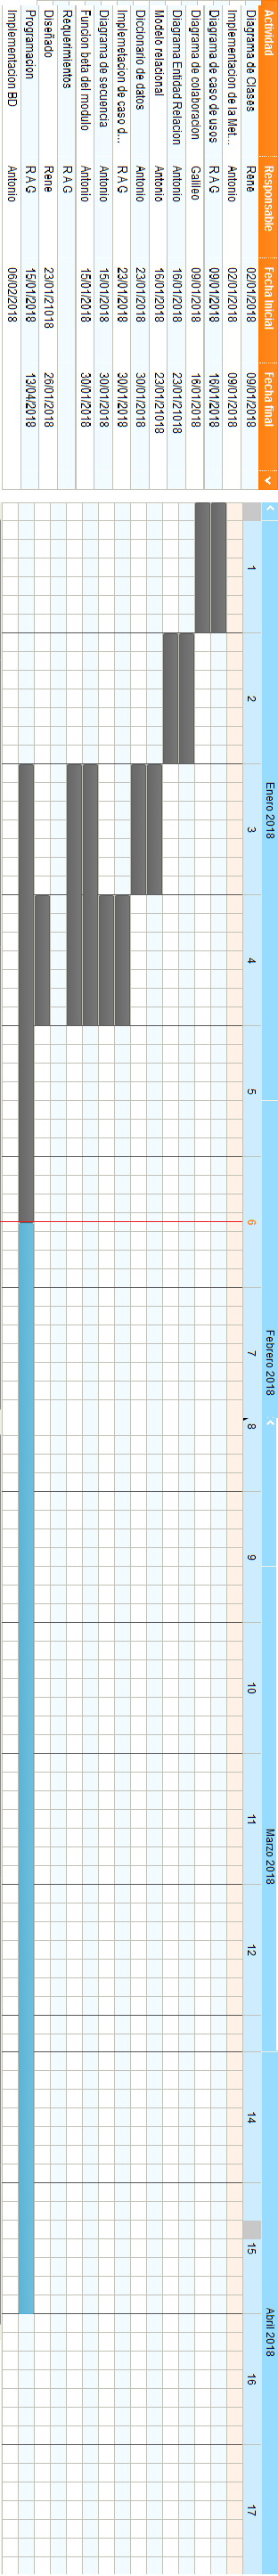
\includegraphics[scale=.15]{gantt.png} 
\end{titlepage}

%%%%%%%%%%%%%%%%%%%%%%%%%%%%%%%%%%%%%%%%%%%%%%%%%%%%%%%%%%%%%%%%%%%%%%%%%%%%%%%%%%%%%%%%%%%%%%%%%%%%%%%%%

\begin{titlepage}
{\Large\bfseries \center   Diagrama pert  \par}
 \vspace{.5cm}
 \justify
Para el diagrama pert primero se realizo la tabla en orden con las actividades a realizar.\\
 Las actividades se ordenan conforme a la prioridad de el desarrollo en el proyecto.
\begin{center}
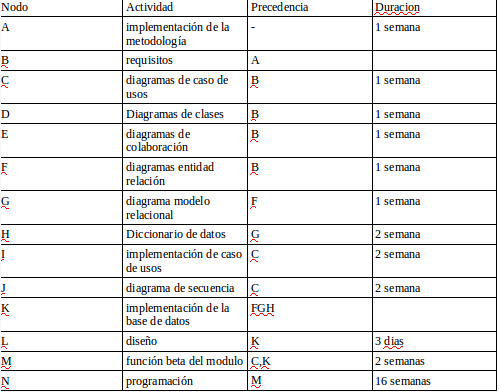
\includegraphics[scale=.6]{2.jpg} 
\end{center}
Mostrar el avance de nuestro proyecto a través del diagrama Pert para tener un buen resultado.
\begin{center}
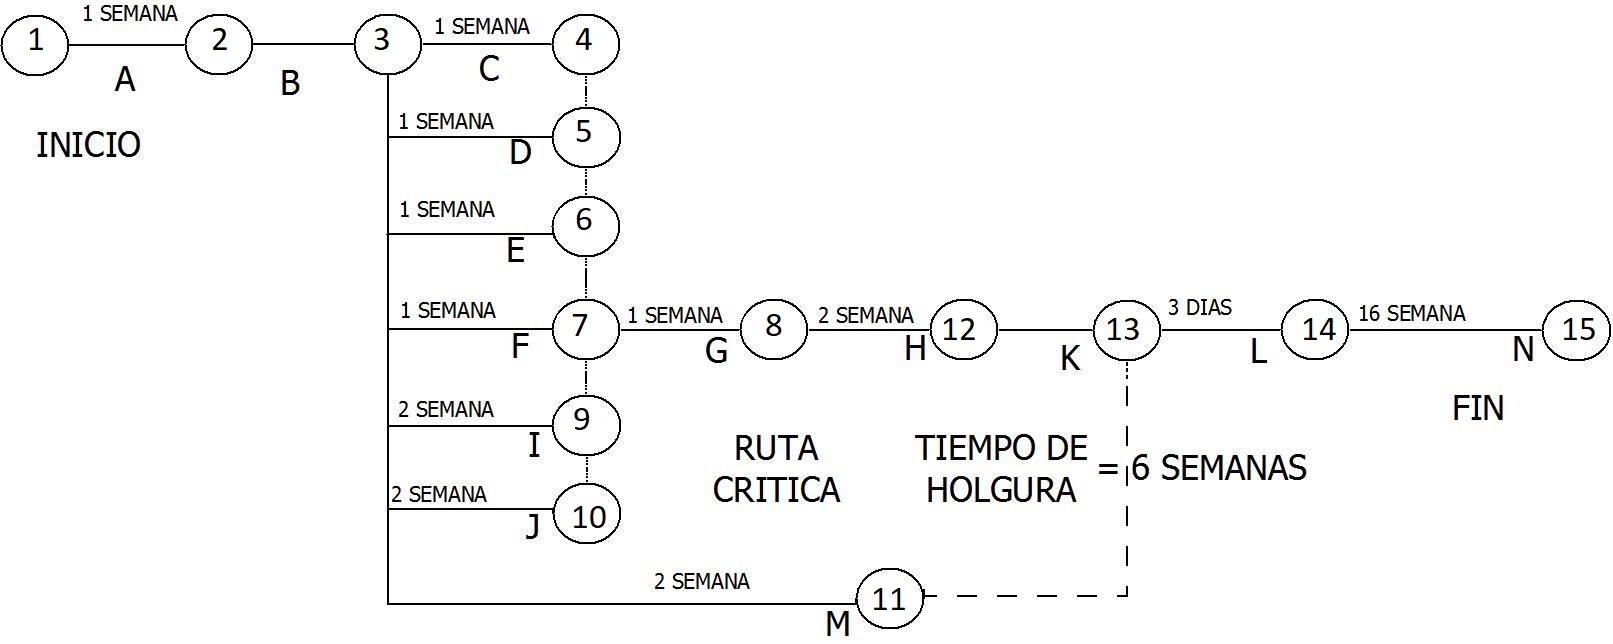
\includegraphics[scale=.3]{3.jpg} 
\end{center}
\end{titlepage}

\begin{titlepage}
\begin{flushleft}


{\Large\bfseries \center   Tipos de Lideres  \par}
 \vspace{.5cm}
  \justify
Líder Técnico: Jose Antonio Garcia Araiza, en el equipo se decidió que el seria el líder técnico ya que el nos aporta mucha información al equipo, nos da ideas y nos asigna las tareas a realizar y el proyecto se pueda realizar de la mejor manera.\\\
 \justify
Líder Socio emocional: Jose Rene De Lima Camacho,se decidió que el seria el líder socio emocional por que muchas veces el da la cara con los profes, y nuestros compañeros, se definiría como la voz del equipo.\\

 
 {\Large\bfseries \center  Normas  \par}
 \vspace{.5cm}
 \justify
Las normas son importantes para seguir una estructura y poder llevar el trabajo en orden, justo por eso nos vimos a la tarea de pensar en 3
normas \par
\vspace{.5cm}
--- Cumplir  con el trabajo en tiempo y forma.\\\

--- participar de forma individual a la toma de decisiones.\\\

--- Asistir a todas las juntas para la toma de decisiones.

\end{flushleft}
\end{titlepage}

%%%%%%%%%%%%%%%%%%%%%%%%%%%%%%%%%%%%%%%%%%%%%%%%%%%%%%%%%%%%%%%%%%%%%%%%%%%%%%%%%%%%%%%%%%%%%%%%%%%%%%%%%

\begin{titlepage}
 
{\Large\bfseries \center Bibliografia \par}
\vspace{1cm}
Septima edicion como aprender a programar en java Deitel\par 
Ingeniria en software septima edicion Ian Sommeryville\par
Systems Analysis and Desing by Dennis Wixom Roth\par 
Analisis de sistema mundo Immanuel Wallesteins
\end{titlepage}

%%%%%%%%%%%%%%%%%%%%%%%%%%%%%%%%%%%%%%%%%%%%%%%%%%%%%%%%%%%%%%%%%%%%%%%%%%%%%%%%%%%%%%%%%%%%%%%%%%%%%%%%%
\end{document}